\documentclass[10pt,letterpaper]{article}

\usepackage[letterpaper,margin=1in]{geometry}
\usepackage[utf8]{inputenc}
\usepackage[T1]{fontenc}
\usepackage{booktabs}
\usepackage{graphicx}
\usepackage{microtype}
\usepackage{url}
\usepackage{hyperref}
\usepackage{float}
\usepackage{natbib}
\usepackage{amsmath}
\usepackage{amssymb}
\usepackage{siunitx}
\usepackage{xcolor}

\emergencystretch=2em

\hypersetup{
    colorlinks=true,
    linkcolor=blue!50!black,
    citecolor=blue!50!black,
    urlcolor=blue!50!black,
    pdftitle={Return-Conservative Distributional Jump Bridges for Financial Disclosure Modeling},
    pdfauthor={Aryan Gupta}
}

\title{Return-Conservative Distributional Jump Bridges for Financial Disclosure Modeling}
\author{
Aryan Gupta\\
\texttt{aryan.cs.app@gmail.com}
}
\date{Preprint, May 2026}

\begin{document}
\maketitle

\begin{abstract}
Financial disclosure models often let event text directly alter every predicted market-response
target, including abnormal return. This is a flexible design, but it can destroy the weaker
cross-sectional ranking signal carried by pre-event market state. We propose the
Return-Conservative Distributional Jump Bridge (RC-DJB), a neural architecture that first estimates
a no-event response distribution and then lets SEC filing text transport volatility, volume, and
predictive uncertainty while imposing a hard firewall on the abnormal-return mean. The constraint is
falsifiable: if disclosure text contains robust near-term return-ranking signal, blocking its direct
return-mean path should hurt; if not, the bridge should improve event-response modeling without
overwriting rank information. On a leakage-controlled public-data study with 7,236 SEC 8-K events,
7,236 matched controls, and 2,463 held-out rows from 98 large U.S. firms, RC-DJB obtains abnormal
return rank IC 0.0546 with 95\% ticker-clustered interval [0.0104, 0.0948]. It is the only tested
model that both beats concat fusion on multi-target MSE by a positive paired interval
(0.0043, [0.0023, 0.0061]) and has a strictly positive ticker-clustered rank-IC interval. Event
bridge interventions increase held-out event-row MSE by 0.0066, 0.0049, and 0.0081 when the bridge
is removed, text is zeroed, or text is shuffled. The result does not establish a complete trading
system; it supports a sharper modeling claim: disclosure text is useful for response-distribution
transport, but directly using it to move the return mean is harmful in this setting.
\end{abstract}

\section{Introduction}

Public disclosures are timed interventions in the market information set. A filing can change
volatility, liquidity, and uncertainty even when its effect on cross-sectional abnormal-return
ranking is weak or unstable. Standard multimodal forecasters typically concatenate price history
and text embeddings, then predict all targets with a shared head. This design asks the same text
representation to explain risk response, volume response, uncertainty, and return ranking. In
financial data, that coupling is a liability: return labels are noisy, text is high dimensional, and
small leakage or overfitting effects can look like alpha.

This paper studies a stricter architectural hypothesis. SEC disclosure text should be allowed to
transport the event-response distribution, but it should not directly overwrite the mean abnormal
return predicted from the no-event market state. We call the resulting model a
Return-Conservative Distributional Jump Bridge (RC-DJB). The model first predicts a no-event
Gaussian response distribution from pre-event price, volume, and market-relative features. It then
uses disclosure text to generate bounded shifts in volatility-jump mean, volume-jump mean, and
predictive log-variance. The abnormal-return mean shift is constrained to zero.

The contributions are:
\begin{enumerate}
    \item A return-conservative distributional bridge architecture for event-driven financial
    modeling.
    \item A leakage-controlled SEC 8-K experiment with matched no-event controls and public
    post-filing market outcomes.
    \item Evidence that blocking direct text-to-return-mean transport recovers statistically
    positive rank IC while preserving response-regression gains over fusion baselines.
    \item Intervention tests showing that the disclosure bridge contributes to event-row MSE even
    though return ranking is intentionally anchored to the no-event state.
\end{enumerate}

\section{Related Work}

Classical event studies estimate abnormal returns around information releases
\citep{fama1969adjustment,brown1985eventstudies,mackinlay1997eventstudies}. RC-DJB keeps this
information boundary but replaces scalar event-window estimation with a neural distributional
response model. The architecture is related to state-space and dynamical-system methods, including
Koopman operators \citep{koopman1931hamiltonian}, neural differential equations
\citep{chen2018neuralode}, structured state-space sequence models \citep{gu2022s4}, and selective
state-space models \citep{gu2023mamba}. Marked point processes model event arrivals
\citep{hawkes1971spectra,mei2017neuralhawkes}; here the disclosure time is observed and the task is
post-event response prediction.

Financial text contains information relevant to prices and fundamentals
\citep{loughran2011liability,cohen2020lazy,araci2019finbert}. Recent work studies multimodal
financial forecasting, financial reasoning benchmarks, and leakage in financial agents
\citep{chen2025camef,islam2023financebench,finrate2026,li2025profitmirage}. Causal Transformer and
G-Transformer estimate counterfactual outcomes in temporal settings
\citep{melnychuk2022causaltransformer,feng2024gtransformer}. RC-DJB differs by imposing a
target-specific architectural restriction: disclosure text may transport response distribution
components, but the abnormal-return mean remains no-event anchored.

\section{Method}

\begin{figure}[H]
\centering

\includegraphics[width=\linewidth]{figures/rc_djb_architecture.pdf}
\caption{RC-DJB first estimates a no-event response distribution from market history. Disclosure
text generates a bounded bridge for risk/liquidity response and predictive uncertainty, but a
return-mean firewall enforces \(\Delta \mu_r=0\).}
\label{fig:architecture}
\end{figure}

\paragraph{Inputs and targets.}
Each sample \(i\) has label start date \(\tau_i\), a 40-trading-day pre-event tensor
\(X_i \in \mathbb{R}^{40 \times 8}\), disclosure embedding \(e_i\), metadata
\(m_i \in \mathbb{R}^{6}\), and target vector \(y_i \in \mathbb{R}^{3}\). The targets are
five-trading-day SPY-adjusted return, realized-volatility jump, and volume jump. The headline
variant uses chunk-pooled BGE-small disclosure embeddings \citep{xiao2023cpack}.

\paragraph{Event-study labels.}
Let \(P_{i,t}\), \(V_{i,t}\), and \(r_{i,t}\) denote adjusted close, volume, and daily close return
for firm \(i\), and let \(r^M_t\) denote the SPY return. The label window
\(\mathcal{W}_i=\{\tau_i,\ldots,\eta_i\}\) starts on the disclosure date for before-close traded-day
filings and on the next traded date otherwise; \(\eta_i\) is the fifth tradable session in the
window. The pre-window
\(\mathcal{P}_i\) is the 20 traded sessions strictly before \(\tau_i\). The implemented targets are
\begin{align}
    y_{i,r}
    &= \frac{P_{i,\eta_i}}{P_{i,\tau_i}} - 1
    - \left(\prod_{t\in\mathcal{W}_i}(1+r^M_t)-1\right),\\
    y_{i,\sigma}
    &= \operatorname{sd}_{t\in\mathcal{W}_i}(r_{i,t})
    - \operatorname{sd}_{t\in\mathcal{P}_i}(r_{i,t}),\\
    y_{i,V}
    &= \frac{|\mathcal{P}_i|}{|\mathcal{W}_i|}
    \frac{\sum_{t\in\mathcal{W}_i} V_{i,t}}{\sum_{t\in\mathcal{P}_i} V_{i,t}} - 1.
\end{align}
Rows are admissible only when their maximum feature date is strictly before the label start,
\(\max\{t:t\in X_i\}<\tau_i\).

\paragraph{No-event distribution.}
A recurrent encoder maps pre-event market history to a latent state:
\begin{equation}
    h_i = \mathrm{GRU}_\theta(X_i) + W_m m_i .
\end{equation}
A bounded gate produces the no-event state \(\tilde{s}_i\), from which the model predicts a
diagonal Gaussian distribution:
\begin{align}
    \tilde{s}_i &= h_i \odot (1 + 0.1 \tanh(g_\theta(h_i,m_i))),\\
    [\mu_{0,i}, \ell_{0,i}] &= f_\theta(\tilde{s}_i,m_i),
\end{align}
where \(\ell_{0,i}\) is log-variance.

\paragraph{Distributional bridge.}
Disclosure text generates a bounded latent state jump and distributional transport:
\begin{align}
    b_i &= B_\theta(e_i),\\
    j_i &= \alpha \tanh(u_\theta(b_i)) \odot \sigma(v_\theta(b_i)),\\
    [\Delta \mu_i, \Delta \ell_i] &= T_\theta(\mathrm{LN}(\tilde{s}_i+j_i), b_i, m_i).
\end{align}
The central architectural constraint is
\begin{equation}
    \Delta \mu_{i,return} = 0.
\end{equation}
Thus,
\begin{equation}
    \mu_{1,i} =
    \mu_{0,i} + [0,\Delta\mu_{i,volatility},\Delta\mu_{i,volume}],
    \qquad
    \ell_{1,i} = \mathrm{clip}(\ell_{0,i}+\Delta\ell_i).
\end{equation}
The model predicts \(p_\theta(y_i)=\mathcal{N}(\mu_{1,i},\mathrm{diag}(\exp(\ell_{1,i})))\).

\paragraph{Objective.}
For target dimension \(k\), the Gaussian negative log likelihood used for probabilistic training
and evaluation is
\begin{equation}
    \mathcal{L}_{NLL}
    = \frac{1}{2NK}\sum_{i=1}^{N}\sum_{k=1}^{K}
    \left[\exp(-\ell_{1,ik})(y_{ik}-\mu_{1,ik})^2+\ell_{1,ik}\right],
    \qquad K=3,\quad \ell_{1,ik}\in[-7,3].
\end{equation}
The pairwise rank regularizer is computed only over real-disclosure pairs in a minibatch:
\begin{equation}
    \mathcal{L}_{rank}
    = \frac{1}{|\mathcal{Q}|}\sum_{(i,j)\in\mathcal{Q}}
    \log\left(1+\exp\left[
    -\operatorname{sign}(y_{i,r}-y_{j,r})
    \frac{\mu_{1,i,r}-\mu_{1,j,r}}{T}
    \right]\right),
\end{equation}
where \(\mathcal{Q}\) contains event pairs with unequal abnormal-return labels and \(T=0.02\).
The supervised term is the weighted Smooth-L1 loss after optional target standardization:
\begin{equation}
    \mathcal{L}_{Huber}
    =
    \frac{1}{NK}\sum_{i=1}^{N}\sum_{k=1}^{K}
    w_k\operatorname{SmoothL1}_{\beta}
    \left(\frac{\mu_{1,ik}-\bar{y}_k}{s_k},
    \frac{y_{ik}-\bar{y}_k}{s_k}\right).
\end{equation}
For bottleneck models with posterior parameters \((\mu^z_i,\ell^z_i)\),
\begin{equation}
    \mathcal{L}_{KL}
    = -\frac{1}{2}\operatorname{mean}_{i,k}
    \left(1+\ell^z_{ik}-(\mu^z_{ik})^2-\exp(\ell^z_{ik})\right).
\end{equation}
The control and consistency penalties are
\begin{align}
    \mathcal{L}_{control}
    &=
    \frac{\sum_i\mathbb{1}\{a_i=0\}\lVert\Delta\mu_i\rVert_2^2}
    {\sum_i\mathbb{1}\{a_i=0\}},\\
    \mathcal{L}_{consistency}
    &= \frac{1}{K}\sum_{k=1}^{K}\operatorname{Var}_i(\Delta\mu_{i,k}),
\end{align}
where \(a_i=1\) for real disclosures and \(a_i=0\) for matched controls.
The full training loss combines target-standardized Huber regression, Gaussian likelihood, control
suppression, bottleneck regularization, bridge sparsity, residual consistency, and rank learning:
\begin{equation}
\mathcal{L} =
\lambda_y\mathcal{L}_{Huber}
+\lambda_n\mathcal{L}_{NLL}
+\lambda_c\mathcal{L}_{control}
+\lambda_{KL}\mathcal{L}_{KL}
+\lambda_s\lVert z_i\rVert_1
+\lambda_v\mathcal{L}_{consistency}
+\lambda_r\mathcal{L}_{rank}.
\end{equation}
Here \(z_i\) is the stored disclosure-bridge latent used for sparsity diagnostics. The main run
uses \(w_y=(3.0,1.0,0.25)\), \(\lambda_n=0.10\), \(\lambda_c=0.35\),
\(\lambda_{KL}=0.01\), \(\lambda_s=0.001\), \(\lambda_v=0.05\), and \(\lambda_r=0.15\).

\section{Data and Leakage Controls}

The experiment uses public SEC EDGAR APIs \citep{secapi}. The sample covers 98 usable large U.S.
firms, SEC 8-K filings from 2020--2025, and public daily prices. Tickers are mapped to CIKs through
the SEC company-tickers file. Filings are read from SEC submissions JSON, including archived
submissions, using \texttt{acceptanceDateTime} and the primary EDGAR document URL. The parser stores
source URL, accession number, accepted timestamp, available timestamp, extracted text, and text
hash.

Daily prices are downloaded from public price endpoints, with SPY used as the market proxy for
abnormal returns. The trading calendar is inferred from observed price rows. Event label windows
start on the same observed trading day for filings accepted before 16:00 ET; filings accepted after
16:00 ET or on non-trading days start on the next observed trading day. Features use only prices
strictly before the label start date. Labels use future returns only as targets. One deterministic same-ticker
no-event control is constructed for each filing, excluding dates within a 10-calendar-day blackout
window around known events.

\begin{table}[H]
\centering
\caption{Main public-data sample.}
\label{tab:substrate}
\begin{tabular}{lr}
\toprule
Artifact & Count \\
\midrule
Usable companies & 98 \\
SEC 8-K events & 7,236 \\
Matched no-event controls & 7,236 \\
Feature rows & 14,472 \\
Public price rows & 159,093 \\
Held-out rows & 2,463 \\
\bottomrule
\end{tabular}
\end{table}

\section{Experiments}

Rows with \(\tau_i \leq\) 2023-12-31 are training rows, rows from 2024 are validation rows, and
later rows are held out. This yields 9,729 training rows, 2,280 validation rows, and 2,463 held-out
rows across 98 held-out tickers and 13 held-out label-start months. The headline RC-DJB checkpoint
is selected by validation loss. All models use fixed seed 29 and are evaluated once on the held-out
split.

Baselines include no-event dynamics, text-only MLP, concat fusion, Counterfactual Event Bottleneck
Transformer (CEBT), Disclosure Operator Transformer (DOT), Event-Jump State Space Model (EJSSM),
and an unconstrained Distributional Jump Bridge (DJB). Confidence intervals use percentile
bootstrap resampling; ticker-clustered intervals resample tickers with replacement. Paired
comparisons use row-paired bootstrap resampling. Rank IC is Spearman correlation between predicted
and realized abnormal return.

\paragraph{Evaluation statistics.}
For model \(m\), the reported multi-target error is
\begin{equation}
    \operatorname{MSE}(m)
    = \frac{1}{NK}\sum_{i=1}^{N}\sum_{k=1}^{K}
    \left(y_{ik}-\hat{y}^{(m)}_{ik}\right)^2 .
\end{equation}
Rank IC is the Spearman correlation between predicted and realized abnormal return:
\begin{equation}
    \operatorname{IC}(m)
    = \rho_P\left(
    \operatorname{rank}(\hat{y}^{(m)}_{1:N,r}),
    \operatorname{rank}(y_{1:N,r})
    \right).
\end{equation}
For a statistic \(S\), bootstrap replicates \(S^{*(1)},\ldots,S^{*(B)}\) form percentile
intervals
\begin{equation}
    \operatorname{CI}_{0.95}(S)
    =
    \left[Q_{0.025}\{S^{*(b)}\}_{b=1}^{B},
    Q_{0.975}\{S^{*(b)}\}_{b=1}^{B}\right],
\end{equation}
The model-level intervals in Table~\ref{tab:main-results} use \(B=1000\). Ticker-clustered
intervals sample tickers with replacement and include all held-out rows for each sampled ticker.
Rank IC uses integer ranks of predicted and realized abnormal returns. Paired MSE comparisons
against RC-DJB use \(B=2000\) row-paired bootstrap replicates and
\begin{equation}
    \Delta_{\operatorname{MSE}}(m)
    = \frac{1}{N}\sum_{i=1}^{N}
    \left[
    \frac{1}{K}\lVert y_i-\hat{y}^{(m)}_i\rVert_2^2
    -
    \frac{1}{K}\lVert y_i-\hat{y}^{RC}_i\rVert_2^2
    \right],
\end{equation}
with rows resampled as matched pairs. Paired rank comparisons use the same joined rows but report
\(\operatorname{IC}(RC)-\operatorname{IC}(m)\).

\paragraph{Probabilistic diagnostics.}
For nominal level \(1-\alpha\), the diagonal Gaussian predictive interval for target \(k\) is
\begin{equation}
    I_{ik}(1-\alpha)
    =
    \left[
    \mu_{1,ik}-z_{1-\alpha/2}\exp(\ell_{1,ik}/2),
    \mu_{1,ik}+z_{1-\alpha/2}\exp(\ell_{1,ik}/2)
    \right],
\end{equation}
and empirical coverage is
\begin{equation}
    \widehat{C}(1-\alpha)
    = \frac{1}{NK}\sum_{i=1}^{N}\sum_{k=1}^{K}
    \mathbb{1}\{y_{ik}\in I_{ik}(1-\alpha)\}.
\end{equation}
Mean predictive standard deviation is
\(\frac{1}{NK}\sum_{i,k}\exp(\ell_{1,ik}/2)\).

\begin{table}[H]
\centering
\caption{Held-out results. MSE is over abnormal return, volatility jump, and volume jump. Intervals
are 95\% ticker-clustered bootstrap intervals.}
\label{tab:main-results}
\small
\begin{tabular}{lrrrr}
\toprule
Model & MSE & MSE CI & Rank IC & Rank IC CI \\
\midrule
No-event & 0.0696 & [0.0519, 0.0936] & -0.0411 & [-0.0840, 0.0016] \\
Concat fusion & 0.0597 & [0.0442, 0.0817] & -0.0182 & [-0.0597, 0.0267] \\
CEBT & 0.0660 & [0.0488, 0.0898] & 0.0463 & [0.0052, 0.0893] \\
DOT & 0.0596 & [0.0449, 0.0804] & -0.0131 & [-0.0510, 0.0291] \\
EJSSM-BGE & 0.0547 & [0.0395, 0.0764] & 0.0099 & [-0.0329, 0.0556] \\
DJB & \textbf{0.0539} & [0.0389, 0.0757] & 0.0128 & [-0.0290, 0.0547] \\
RC-DJB & 0.0554 & [0.0400, 0.0776] & \textbf{0.0546} & [0.0104, 0.0948] \\
\bottomrule
\end{tabular}
\end{table}

\begin{table}[H]
\centering
\caption{Paired comparisons against RC-DJB. Positive MSE values mean RC-DJB has lower MSE. Positive
rank values mean RC-DJB has higher rank IC.}
\label{tab:paired}
\small
\begin{tabular}{lrrrr}
\toprule
Baseline & MSE Diff. & 95\% CI & Rank IC Diff. & 95\% CI \\
\midrule
No-event & 0.01417 & [0.01150, 0.01747] & 0.0956 & [0.0412, 0.1504] \\
Concat fusion & 0.00427 & [0.00230, 0.00612] & 0.0728 & [0.0197, 0.1249] \\
CEBT & 0.01057 & [0.00825, 0.01311] & 0.0083 & [-0.0500, 0.0668] \\
DOT & 0.00418 & [0.00180, 0.00638] & 0.0677 & [0.0186, 0.1180] \\
EJSSM-BGE & -0.00076 & [-0.00163, 0.00005] & 0.0447 & [-0.0072, 0.0952] \\
\bottomrule
\end{tabular}
\end{table}

\paragraph{Bridge diagnostics.}
The response-transport statistic for group \(c\in\{0,1\}\) is
\begin{equation}
    T_c
    =
    \operatorname{mean}_{i:a_i=c,k}\left|\Delta\mu_{i,k}\right|,
\end{equation}
where \(c=1\) denotes real 8-K rows and \(c=0\) denotes controls. Latent bridge AUC uses the score
\(s_i=\operatorname{mean}_k|z_{i,k}|\) to classify real disclosures against matched controls, with
average ranks used for tied scores.

\begin{table}[H]
\centering
\caption{RC-DJB diagnostics on the held-out split.}
\label{tab:diagnostics}
\begin{tabular}{lr}
\toprule
Diagnostic & Value \\
\midrule
Gaussian NLL & -2.2864 \\
Observed 80\% interval coverage & 0.9011 \\
Observed 95\% interval coverage & 0.9602 \\
Mean predictive standard deviation & 0.1302 \\
Mean response transport, real 8-Ks & 0.0358 \\
Mean response transport, controls & 0.0073 \\
Latent bridge AUC, events vs. controls & 0.6038 \\
\bottomrule
\end{tabular}
\end{table}

\paragraph{Intervention definitions.}
The no-bridge intervention is the implementation's no-jump forward pass: it sets the bridge state
jump, bridge hidden state, mean delta, and log-variance delta to zero, so \(\mu_1=\mu_0\) and
\(\ell_1=\ell_0\). The zero-text intervention replaces \(e_i\) with the zero vector before the
forward pass. The shuffled-text intervention applies one deterministic held-out permutation of
disclosure embeddings. For RC-DJB, \(\Delta\mu_{return}=0\) in every variant, so abnormal-return
point predictions and rank IC are invariant to these bridge interventions.

\begin{table}[H]
\centering
\caption{RC-DJB intervention tests. Rank IC is unchanged by bridge interventions because the
return-mean firewall fixes the abnormal-return point prediction to the no-event mean.}
\label{tab:interventions}
\small
\begin{tabular}{lrrrrr}
\toprule
Variant & All MSE & Event MSE & Event NLL & Rank IC & Bridge AUC \\
\midrule
Full RC-DJB & \textbf{0.0554} & \textbf{0.0843} & \textbf{-2.2115} & 0.0546 & 0.6038 \\
No bridge & 0.0586 & 0.0909 & -2.1204 & 0.0546 & 0.5000 \\
Zero text & 0.0578 & 0.0892 & -2.1886 & 0.0546 & 0.4843 \\
Shuffled text & 0.0597 & 0.0924 & -2.1765 & 0.0546 & 0.5057 \\
\bottomrule
\end{tabular}
\end{table}

\begin{table}[H]
\centering
\caption{Paired event-row MSE stress tests. Positive values mean full RC-DJB has lower event-row MSE
than the intervention.}
\label{tab:intervention-paired}
\small
\begin{tabular}{lrr}
\toprule
Intervention & Event MSE increase & 95\% paired CI \\
\midrule
No bridge & 0.0066 & [0.0043, 0.0093] \\
Zero text & 0.0049 & [0.0027, 0.0073] \\
Shuffled text & 0.0081 & [0.0051, 0.0117] \\
\bottomrule
\end{tabular}
\end{table}

\begin{figure}[H]
\centering

\includegraphics[width=\linewidth]{figures/rc_djb_pareto_frontier.pdf}
\caption{RC-DJB occupies a different point on the response/ranking tradeoff: EJSSM and DJB have
lower point MSE, while RC-DJB is the only tested low-error model with a strictly positive
ticker-clustered rank-IC interval.}
\label{fig:pareto}
\end{figure}

\begin{figure}[H]
\centering
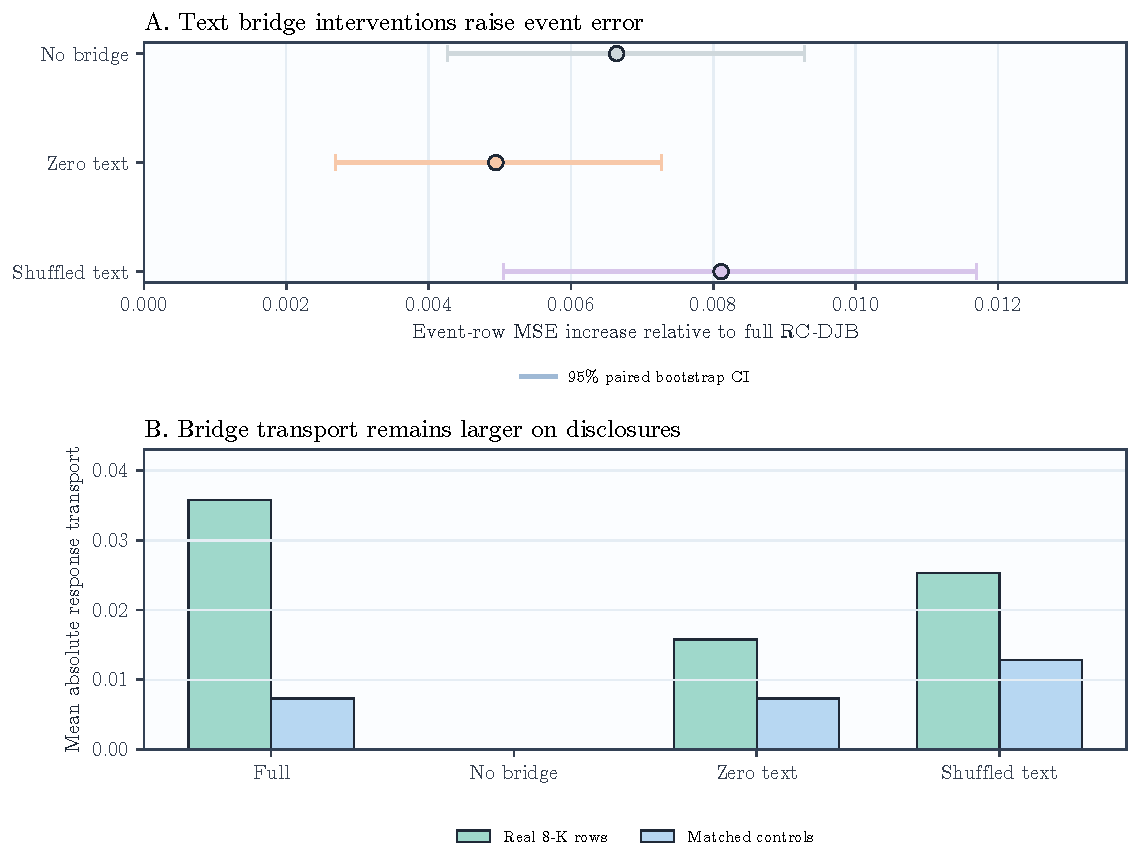
\includegraphics[width=\linewidth]{figures/rc_djb_intervention_story.pdf}
\caption{Interventions show that the disclosure bridge matters for event-response error. Rank IC
does not move under text interventions because the return-mean firewall prevents direct
text-to-return overwriting.}
\label{fig:interventions}
\end{figure}

\begin{figure}[H]
\centering

\includegraphics[width=\linewidth]{figures/rc_djb_monthly_rank_heatmap.pdf}
\caption{Monthly event-rank IC over held-out real 8-K rows. The model-level rank result is not
uniform across months, but RC-DJB has a more positive held-out pattern than fusion and unconstrained
event-mean transport baselines.}
\label{fig:rank-heatmap}
\end{figure}

\section{Findings}

\paragraph{Return-mean conservation recovers rank signal.}
RC-DJB obtains rank IC 0.0546 with ticker-clustered interval [0.0104, 0.0948]. In contrast,
concat fusion, DOT, EJSSM-BGE, and unconstrained DJB all have rank intervals crossing zero. CEBT
also has positive rank IC, but its MSE is much worse than RC-DJB.

\paragraph{The bridge improves response modeling without moving return means.}
RC-DJB improves paired MSE over concat fusion by 0.0043 and over DOT by 0.0042. Removing the bridge
raises event-row MSE by 0.0066; zeroing or shuffling text raises event-row MSE by 0.0049 and
0.0081. These changes occur even though abnormal-return predictions are unchanged by construction,
which means the bridge is acting through volatility, volume, and uncertainty transport.

\paragraph{There is a real response/ranking tradeoff.}
EJSSM-BGE and unconstrained DJB achieve lower point MSE than RC-DJB, but their rank IC intervals
include zero. RC-DJB is therefore not a universal winner; it is a Pareto-frontier point that
prioritizes statistically reliable ranking while keeping response error below fusion baselines.
This tradeoff is the main empirical evidence for the return firewall.

\paragraph{The likelihood result is competitive but not decisive.}
RC-DJB has Gaussian NLL -2.2864, close to EJSSM-BGE's -2.2839. The paired NLL difference against
EJSSM-BGE is small and not statistically decisive. The likelihood evidence supports the bridge as
competitive; the distinctive result is the combination of positive rank IC and response-error
improvement over fusion baselines.

\section{Reproducibility}

The artifact records configurations, seeds, processed event metadata, text hashes, price rows,
feature metadata, checkpoints, predictions, table CSVs, and figure outputs used for the reported
results. Tests cover timestamp gating, after-hours label starts, feature leakage rejection, control
construction, deterministic cached tensors, finite model losses, probabilistic loss integration,
and evaluation leakage guards. Labels are computed only from future price windows and are never
included in model inputs.

\section{Limitations}

The study has several limitations. The universe is large-cap biased and may contain survivorship
effects, ticker-history issues, and 8-K item-mix sensitivity. The price source is public daily data
rather than CRSP or intraday trades and quotes. Abnormal returns are SPY-adjusted rather than
factor-model residuals. BGE-small is a general-purpose encoder, and filings are represented by
chunk mean pooling rather than a trained long-document financial encoder. Rank IC is statistically
positive but economically small; transaction costs, capacity, and portfolio construction are outside
the scope of this study. The return firewall is an architectural and predictive constraint, not
structural causal identification.

\section{Ethics and Use}

This paper studies event representations using public filings and public daily prices. The results
do not constitute trading recommendations. The artifact is intended to support leakage auditing,
independent reproduction, and falsification of the empirical claims.

\section{Conclusion}

RC-DJB shows that the route by which disclosure text enters a financial event model matters. Letting
text directly move the abnormal-return mean is not necessary for response modeling and appears to
harm ranking in this setting. A return-conservative distributional bridge obtains positive
held-out rank IC while still improving multi-target event-response MSE over concat fusion and DOT.
The evidence supports a more precise architecture principle for disclosure modeling: use text to
transport response risk, liquidity, and uncertainty, but keep near-term return ranking anchored to
the no-event market state unless stronger evidence justifies crossing that boundary.

\bibliographystyle{plainnat}
\bibliography{references}

\end{document}
